\documentclass{article}
\usepackage{amsmath}
\usepackage{graphicx}
\usepackage{caption}
\usepackage{natbib}
\usepackage{float}
\title{Latex Document}
\author{Keshav Mishra}
\date{October 15, 2024}

\begin{document}
	\maketitle
	\section{Simple Text}
	In March 2006, Congress raised that ceiling an additional \$0.79 trillion to
	\$8.97 trillion, which is approximately 68\% of GDP. As of October 4, 2008, the
	“Emergency Economic Stabilization Act of 2008” raised the current debt
	ceiling to \$11.3 trillion.
	\section{Mathematical Expression}
	
	\begin{equation}
		\mathbf{h}_v^k \leftarrow \sigma \left( \mathbf{W} \cdot \text{MEAN} \left( \{ \mathbf{h}_v^{k-1} \} \cup \{ \mathbf{h}_{u}^{k-1} \, , \, \forall u \in \mathcal{N}(v) \} \right) \right)
		\label{eq:equation1}
	\end{equation}
	\begin{equation}
		\text{AGGREGATE}_{k}^{\text{pool}} = \max \left( \{ \sigma \left( \mathbf{W}_{\text{pool}} \mathbf{h}_{u_i}^{k} + \mathbf{b} \right) \, , \, \forall u_i \in \mathcal{N}(v) \} \right)	
		\label{eq:equation2}    
	\end{equation}	
	\ref{eq:equation1} tells us that an important distinction between this convolutional aggregator
	and our other proposed aggregators is that it does not perform the concatenation operation i.e., the convolutional aggregator does concatenate the node’s previous layer. As discussed in \cite{10.1145/1150402.1150479}.\\
	\ref{eq:equation2} tells us that the final aggregator we examine is both symmetric and trainable. In this
	pooling approach, each neighbor’s vector is independently fed through a fully-connected neural
	network. As is given in \cite{10.1145/3219819.3219890}.
	\section{Image}
	In Figure \ref{fig: Landscape's_image}, we can see a beautiful scenery of nature.
	\begin{figure}[H]
		\centering
		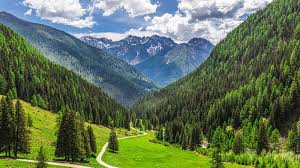
\includegraphics[width=0.5\textwidth]{landscape.jpg}
		\caption{A beautiful scenery of mountain}
		\label{fig: Landscape's_image}
	\end{figure}
	\section{Educational Qualifications}
	\begin{table}[H]
		\centering
		\caption{Educational Qualifications}
		\begin{tabular}{|c|c|c|c|}
			\hline
			\textbf{Degree} & \textbf{Name of School/College} & \textbf{Marks in CGPA or Percentage} & \textbf{Year of Passing} \\
			\hline
			B.Tech & IIT Bhilai & 9.71 & 2024 \\
			\hline
			12th & Adarsh Public School & 95.2\% & 2023 \\
			\hline
			10th & Jesus and Mary Convent School & 91.3\% & 2021 \\
			\hline
		\end{tabular}
	\end{table}
	\bibliographystyle{plain}
	\bibliography{1}
\end{document}
